\documentclass[a4paper]{ltjsarticle}

\usepackage{amsmath} % 数式を記述するためのパッケージ
\usepackage{graphicx} % 画像を挿入するためのパッケージ
\usepackage{url} % URLを記述するためのパッケージ
\usepackage{here} % 図表をその場所に表示するためのパッケージ
\usepackage{luacode} % ソースコードを記述するためのパッケージ
\usepackage{titling} % タイトルをカスタマイズするためのパッケージ
\usepackage{fancyhdr} % ヘッダーをカスタマイズするためのパッケージ
\usepackage{siunitx}
\usepackage{multirow}
\usepackage{bigdelim}
\usepackage{amssymb}
\usepackage{listings}
\usepackage{xcolor}
\usepackage{multicol}
\usepackage[subrefformat=parens]{subcaption}

\definecolor{codegreen}{rgb}{0,0.6,0}
\definecolor{codegray}{rgb}{0.5,0.5,0.5}
\definecolor{codepurple}{rgb}{0.58,0,0.82}
\definecolor{backcolour}{rgb}{0.95,0.95,0.92}

\lstdefinestyle{mystyle}{
    backgroundcolor=\color{backcolour},   
    commentstyle=\color{codegreen},
    keywordstyle=\color{blue},
    numberstyle=\tiny\color{codegray},
    stringstyle=\color{codepurple},
    basicstyle=\ttfamily\footnotesize,
    breakatwhitespace=false,         
    breaklines=true,                 
    captionpos=b,                    
    keepspaces=true,                 
    numbers=left,                    
    numbersep=5pt,                  
    showspaces=false,                
    showstringspaces=false,
    showtabs=false,                  
    tabsize=2,
    title=\lstname
}
\lstset{style=mystyle}


\preauthor{\begin{flushright}} % authorを右寄せにする
\postauthor{\end{flushright}}
\predate{\begin{flushright}} % dateを右寄せにする
\postdate{\end{flushright}}

\pagestyle{fancy}
\lhead{電気電子情報実験・演習第一 A2実験レポート}
\rhead{03240403 井上聡士}
\cfoot{\thepage}
\renewcommand{\headrulewidth}{0pt}


\title{電気電子情報実験・演習第一 A2実験レポート}
\author{電子情報工学科 \ 03240403 井上聡士}
\date{2024年7月11日}


\begin{document}
\maketitle % タイトルページを表示する
\tableofcontents
\clearpage

\section{オフセット調整}
まず、オペアンプのオフセット調整を行った。
オペアンプのオフセットとは、入力が0のときに出力に生じる電圧のことで、理想的には$\SI{0}{V}$であるべきだが、実際は$\SI{0}{V}$からずれてしまう。
これは、オペアンプを構成するトランジスタの特性によるものである。
オペアンプは対称的なトランジスタの差動増幅回路で構成されており、トランジスタの特性が異なると、出力にオフセットが生じる\cite{Opamp offset}。
\begin{figure}[htbp]
    \centering
    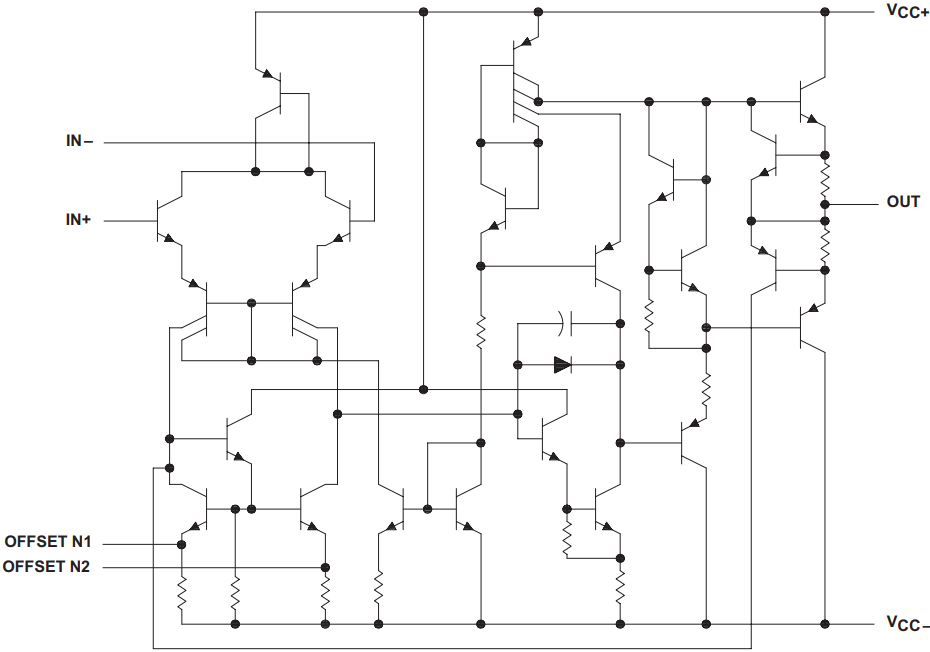
\includegraphics[width=0.6\columnwidth]{./images/opamp_uA741.png}
    \caption{使用したオペアンプ\mu A741の回路図}
    \label{fig:uA741_circuit}
\end{figure}
実際、今回使用したオペアンプ\mu A741も、対称的なトランジスタからなることがわかる(図\ref{fig:uA741_circuit})\cite{uA741}。

実際にオペアンプを調整すると、調整しても電圧が数V程度時間により変化する現象が観測された。
これは、オペアンプの増幅率の高さとノイズに起因するものだと考えられる。
使用したオペアンプ\mu A741は、低周波数での増幅率は$\SI{106}{dB}$、すなわち$10^5$倍以上となっており、数十$\si{\micro V}$程度の入力側のノイズが出力では数$\si{V}$程度に増幅されてしまう\cite{uA741}。
そのため、オフセットを調整してもノイズにより0からずれることがあると考えられる。

\section{反転増幅回路}
\subsection{理論値の計算} \label{sec:invertamp_theory}
\begin{figure}[htbp]
    \centering
    \begin{minipage}{0.48\columnwidth}
        \centering
        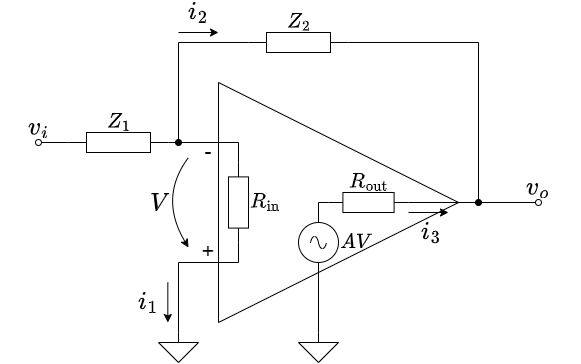
\includegraphics[width=0.95\columnwidth]{./images/invertamp.png}
        \subcaption{回路図}
        \label{fig:invertamp_circuit}
    \end{minipage}
    \begin{minipage}{0.48\columnwidth}
        \centering
        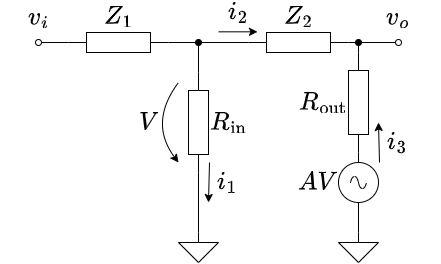
\includegraphics[width=0.95\columnwidth]{./images/invertamp_c.png}
        \subcaption{等価回路図}
        \label{fig:invertamp_eqcircuit}
    \end{minipage}
    \caption{反転増幅回路}
\end{figure}
図\ref{fig:invertamp_circuit}、\ref{fig:invertamp_eqcircuit}は反転増幅回路の回路図とその等価回路である。
入力インピーダンス$R_\text{in}$が十分に大きく($R_\text{in}\rightarrow\infty$)、出力インピーダンス$R_\text{out}$が十分に小さく($R_\text{out}\rightarrow0$)なるように設計されているとき、等価回路の$R_\text{in}$は切断($i_1=0$)、$R_\text{out}$は短絡とみなすことが出来る。
このとき、オペアンプの増幅率を$A$として、以下のような式が成立する。
\begin{align}
    v_i - Z_1i_2 &= -V \\
    v_i - (Z_1+Z_2)i_2 &= v_o \\
    v_o = AV
\end{align}
これを解くと、$\frac{Z_2}{Z_1}=\alpha$として、
\begin{align}
    \frac{v_o}{v_i} &= -\frac{AZ_2}{AZ_1+Z_1+Z_2} \nonumber \\
    &= -\frac{A\frac{Z_2}{Z_1}}{A+\left( 1+\frac{Z_2}{Z_1} \right)} \nonumber \\
    &= -\frac{A\alpha}{A+1+\alpha}
\end{align}
となる。
今、$|A| >> \max(1, \alpha)$のとき、
\begin{equation}
    \frac{v_o}{v_i} \rightarrow -\alpha
\end{equation}
で、$|A| << 1$のとき、
\begin{equation}
    \frac{v_o}{v_i} \rightarrow -A\frac{\alpha}{1+\alpha}
\end{equation}
となる。
この$\alpha$は反転増幅回路の増幅率であり、今回$\alpha=\SI{20}{dB}=10,\,\SI{40}{dB}=100$となるように設定する。
このとき、$\alpha >> 1$と近似でき、$|A|<<1$のとき、$\frac{v_o}{v_i}\rightarrow-A$となる。
すなわち、$A$が大きい領域では一定値を、$A$が小さい領域では$A$に張り付いて変化する。

\subsection{実測値}
\begin{figure}[htbp]
    \centering
    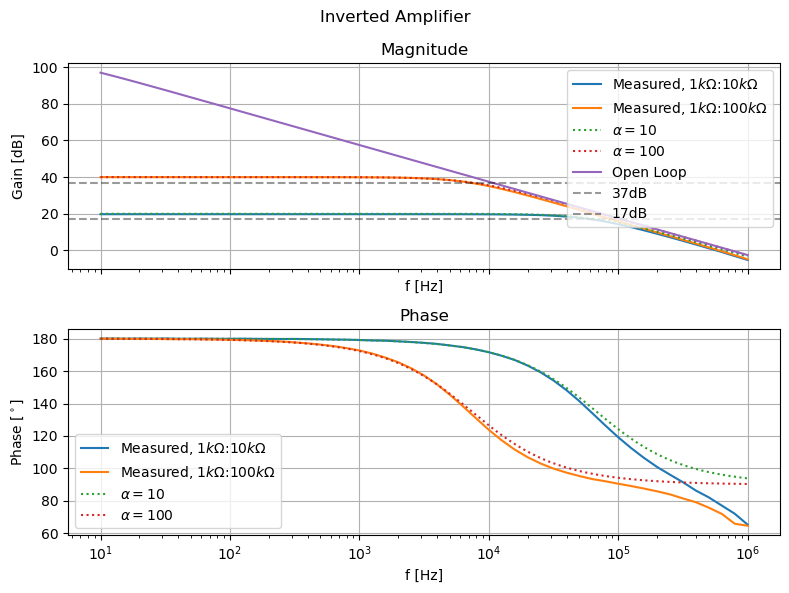
\includegraphics[width=0.8\columnwidth]{./images/invertamp_bode.png}
    \caption{反転増幅回路の周波数応答}
    \label{fig:invertamp_bode}
\end{figure}
図\ref{fig:invertamp_bode}は反転増幅回路の周波数応答の実測値(実線)と理論値(破線)である。
開ループの増幅率$A(s)$は、データシートに乗っていた数値から、Low Passの$A(s)=\frac{A_0}{1+\frac{s}{\omega_P}}$、ただし$A_0=\SI{106}{dB},\,\omega_P=\SI{3.8}{Hz}$として近似した。
振幅特性については、理論値と非常によく一致しており、低周波では意図した増幅率$\alpha$、高周波では$A$に張り付いて$\SI{-20}{dB/dec}$で減少した。


一方、位相特性については、$A(s)$が比較的大きい低周波領域では一致しているが、周波数が大きくなると一致しないことが分かった。
これは、$\alpha$が$s$に依存しており、寄生インダクタンスや寄生容量が存在することを示している。
特に、高周波での影響が大きいことから、寄生インダクタンスが大きいと考えられる。
\begin{figure}[htbp]
    \centering
    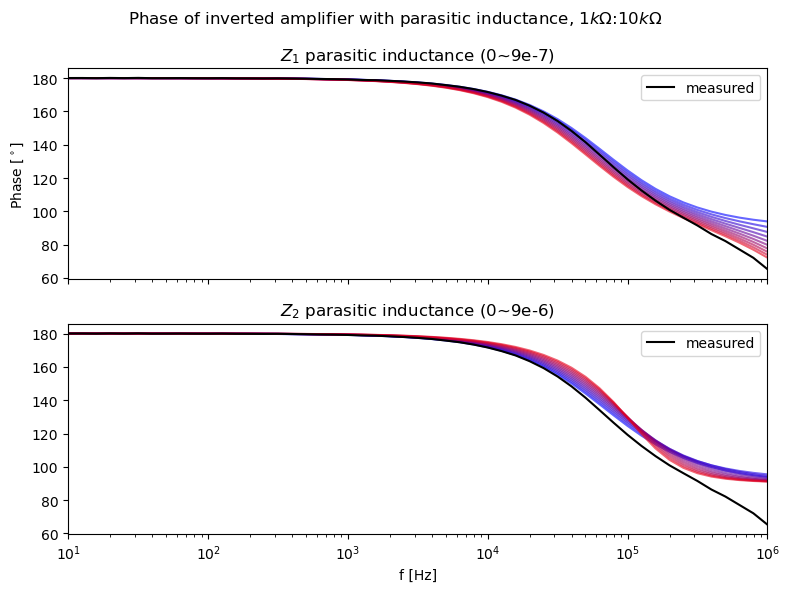
\includegraphics[width=0.8\columnwidth]{./images/invertamp_bode_pi.png}
    \caption{反転増幅回路の位相特性の寄生インダクタンスによる変化}
    \label{fig:invertamp_bode_pi}
\end{figure}

図\ref{fig:invertamp_bode_pi}は$\SI{20}{dB}$ゲインの、$Z_1,\,Z_2$の寄生インダクタンスを変化させた時の位相特性である。
青色に近いほど寄生インダクタンスは小さく($\SI{0}{H}$)、赤色では大きくなる($Z_1$は$\SI{9E-7}{H}$, $Z_2$は$\SI{9E-6}{H}$)。
このように、寄生インダクタンスが存在すると思われる。
実際にフィッティングすると、$Z_1$には$\SI{4E-19}{H}$、$Z_2$には$\SI{8E-7}{H}$程度のインダクタンスが存在すると推定される。

\subsection{遮断周波数}
$\alpha=\SI{20}{dB}$の遮断周波数は、$\SI{17}{dB}$との交点で、$f_1=\SI{6E4}{Hz}$だった。
$\alpha=\SI{40}{dB}$の遮断周波数は、$\SI{37}{dB}$との交点で、$f_2=\SI{7E3}{Hz}$だった。
また、$\alpha$と$f$はほぼ反比例の関係にあり、その積は一定で$\SI{7E5}{Hz}$程度であり、開ループ特性が$\SI{0}{dB}$となるユニティゲイン周波数$f_u$とほぼ一致した。

\section{非反転増幅回路}
\subsection{理論値の計算}
\begin{figure}[hbp]
    \centering
    \begin{minipage}{0.48\columnwidth}
        \centering
        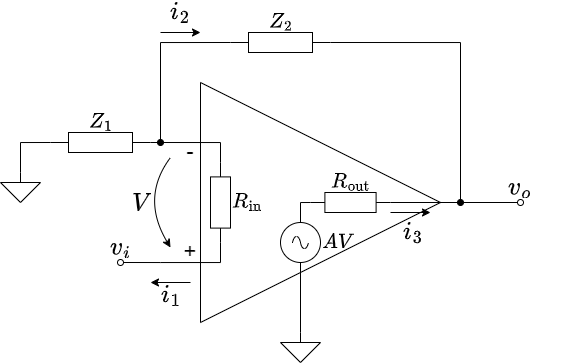
\includegraphics[width=0.95\columnwidth]{./images/noninvertamp.png}
        \subcaption{回路図}
        \label{fig:noninvertamp_circuit}
    \end{minipage}
    \begin{minipage}{0.48\columnwidth}
        \centering
        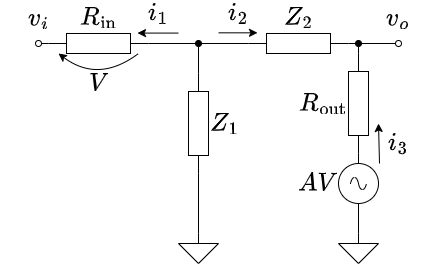
\includegraphics[width=0.95\columnwidth]{./images/noninvertamp_c.png}
        \subcaption{等価回路図}
        \label{fig:noninvertamp_eqcircuit}
    \end{minipage}
    \caption{非反転増幅回路}
\end{figure}
図\ref{fig:noninvertamp_circuit}、\ref{fig:noninvertamp_eqcircuit}は非反転増幅回路の回路図とその等価回路である。
反転増幅回路と同様、$R_\text{in}$は切断($i_1=0$)、$R_text{out}$は短絡と考えてよいので、以下の式が成立する。
\begin{align}
    V &= v_1 + Z_1i_2 \\
    -Z_1i_2 - Z_2i_2 &= AV \\
    v_o &= -Z_1i_2 - Z_2i_2
\end{align}
このとき、$\beta=\frac{Z_1+Z_2}{Z_1}$とすると、
\begin{equation}
    \frac{v_o}{v_i} = \frac{A\beta}{A + \beta}
\end{equation}
となり、$|A|>>\beta$のとき$\frac{v_o}{v_i}\rightarrow\beta$、$|A|<<\beta$のとき$\frac{v_o}{v_i}\rightarrow A$となる。

\subsection{実測値}
\begin{figure}[htbp]
    \centering
    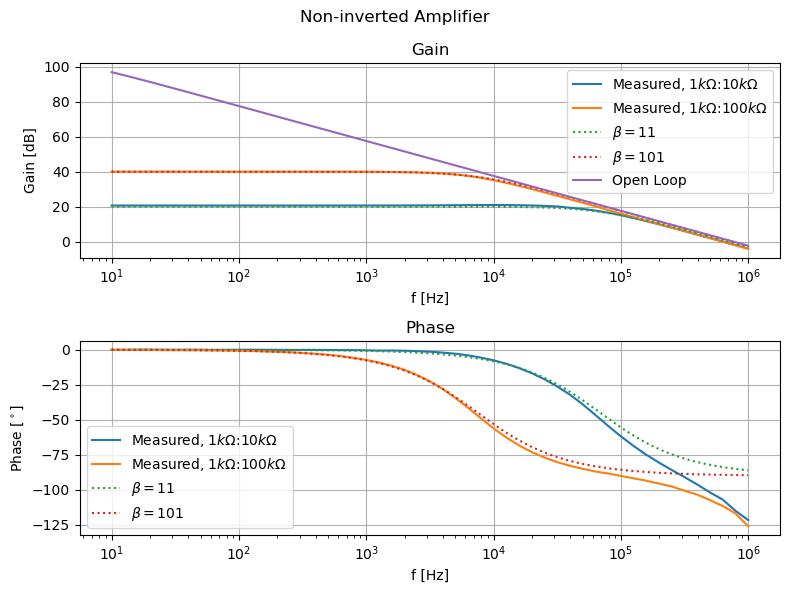
\includegraphics[width=0.8\columnwidth]{./images/noninvertamp_bode.png}
    \caption{非反転増幅回路の周波数応答}
    \label{fig:noninvertamp_bode}
\end{figure}
図\ref{fig:noninvertamp_bode}は非反転増幅回路の周波数応答の実測値(実線)と理論値(破線)である。
反転増幅回路と同様、振幅特性については理論値と非常によく一致しており、低周波では意図した増幅率$\beta$、高周波では$A$に張り付いて$\SI{-20}{dB/dec}$で減少した。

また、位相特性についても、$A(s)$が比較的大きい低周波領域では一致しているが、周波数が大きくなると一致しないことが分かった。
反転増幅回路とほぼ同様なことから、これも寄生インダクタンスによるものだと思われる。

\subsection{遮断周波数}
$\beta=\SI{20}{dB}$の遮断周波数は、$\SI{17}{dB}$との交点で、$f_1=\SI{6E4}{Hz}$だった。
$\beta=\SI{40}{dB}$の遮断周波数は、$\SI{37}{dB}$との交点で、$f_2=\SI{7E3}{Hz}$だった。
また、$\alpha$と$f$はほぼ反比例の関係にあり、その積は一定で$\SI{7E5}{Hz}$程度であり、開ループ特性が$\SI{0}{dB}$となるユニティゲイン周波数$f_u$とほぼ一致した(GB積一定)。

\section{微分回路}
\subsection{理論値の計算}
$Z_1$を抵抗$R_r$とキャパシタ$C_r$の直列回路、$Z_2$を抵抗$R_f$とキャパシタ$C_f$の並列回路として、微分回路を構成した。
すなわち、
\begin{equation*}
    Z_1 = R_r + \frac{1}{sC_r},\quad Z_2 = \frac{R_f}{1+sR_fC_f}
\end{equation*}
とした。
このとき、微分回路は反転増幅回路の$Z$を変えたものとみなせて、
\begin{equation}
    \alpha = \frac{Z_2}{Z_1} = \frac{sR_fC_r}{(1+sR_fC_f)(1+sR_rC_r)}
\end{equation}
となる。
今、$\omega_1 = \frac{1}{R_rC_r}$、$\omega_2 = \frac{1}{R_fC_f}$とすると、
\begin{equation}
    \alpha = \frac{sR_fC_r}{\left( 1+\frac{s}{\omega_1} \right)\left( 1+\frac{s}{\omega_2} \right)}
\end{equation}
となる。

$\omega_1 << \omega_2$のとき、この式は以下のように近似できる。
\begin{equation}
    \alpha \approx \begin{cases}
        sR_fC_r & (|s| < \omega_1) \\
        \frac{R_f}{R_r} & (\omega_1 < |s| < \omega_2) \\
        \frac{1}{R_rC_f}\frac{1}{s} & (\omega_2 < |s|)
    \end{cases}
\end{equation}
すなわち、増幅器のゲイン$A(s)$が十分大きいとき、低周波数帯では微分回路、中周波数帯では反転増幅回路、高周波数帯では積分回路として振る舞う。

\subsection{実測値}
設計にあたり、以下の値の抵抗・キャパシタを使用した。
\begin{align*}
    R_r &= \SI{9.981}{k\ohm},\quad R_f = \SI{99.09}{k\ohm} \\
    C_r &= \SI{218.6}{nF},\quad C_f = \SI{214}{pF}
\end{align*}
このとき、$f_1=2\pi\omega_1 = \SI{73}{Hz}$、$f_2=2\pi\omega_2 = \SI{7.5}{kHz}$となる。
\begin{figure}[htbp]
    \centering
    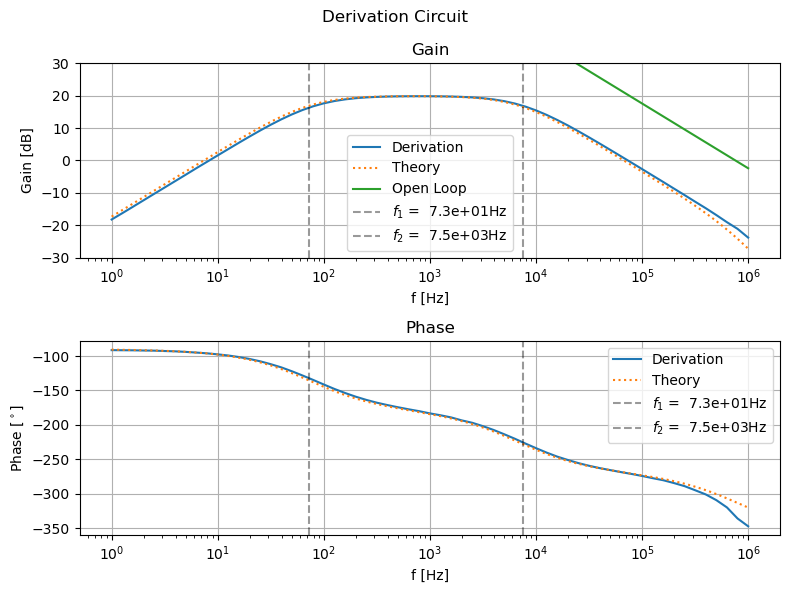
\includegraphics[width=0.8\columnwidth]{./images/dervamp_bode.png}
    \caption{微分回路の周波数応答}
    \label{fig:dervamp_bode}
\end{figure}
図\ref{fig:dervamp_bode}は微分回路の周波数応答の実測値(実線)と理論値(破線)である。
開ループ特性(緑色)と比べると、$\alpha(s)$はどの領域においても十分小さく、上で求めた近似(反転増幅回路の$-\alpha$の近似)が成立する領域にあった。
このとき、理論値と実測値は振幅特性・位相特性共に非常によく一致していた。
唯一、高周波領域で多少の位相のずれはあるが、これは反転増幅回路と同様に寄生インダクタンスの存在によるものだと思われる。

\subsection{ステップ応答}
\begin{figure}[htbp]
    \centering
    \begin{minipage}{0.48\columnwidth}
        \centering
        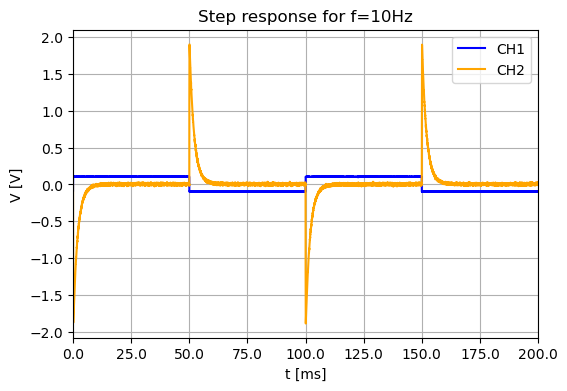
\includegraphics[width=0.95\columnwidth]{./images/dervamp_10Hz.png}
        \subcaption{$f=\SI{10}{Hz}$の方形波応答}
    \end{minipage}
    \begin{minipage}{0.48\columnwidth}
        \centering
        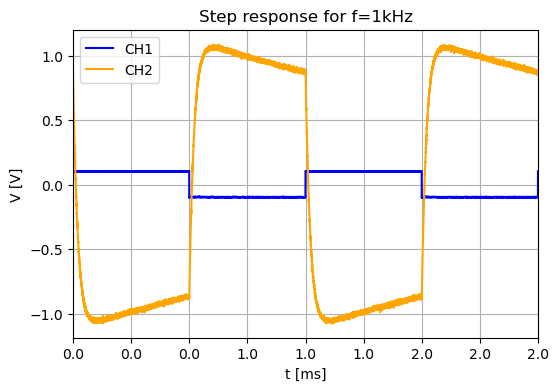
\includegraphics[width=0.95\columnwidth]{./images/dervamp_1kHz.png}
        \subcaption{$f=\SI{1}{kHz}$の方形波応答}
    \end{minipage} \\
    \begin{minipage}{0.48\columnwidth}
        \centering
        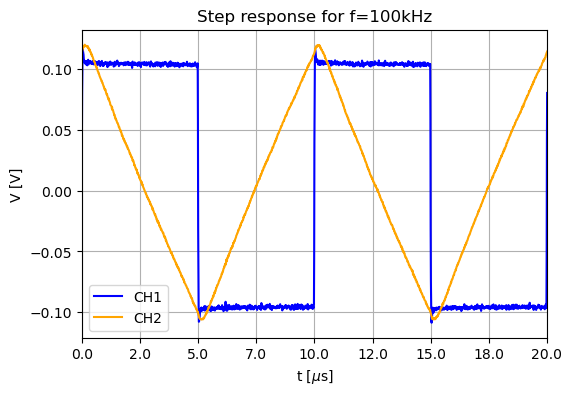
\includegraphics[width=0.95\columnwidth]{./images/dervamp_100kHz.png}
        \subcaption{$f=\SI{100}{kHz}$の方形波応答}
    \end{minipage}
    \caption{微分回路の各周波数帯での方形波応答}
    \label{fig:dervamp_square}
\end{figure}
図\ref{fig:dervamp_square}は微分回路の各周波数帯での方形波応答である。
図\ref{fig:dervamp_bode}を参照すると、$f=\SI{10}{Hz}$のときは微分回路、$f=\SI{1}{kHz}$のときは反転増幅回路、$f=\SI{100}{kHz}$のときは積分回路として振る舞うが、それぞれの実際の方形波応答はこの通りである。
$f=\SI{10}{Hz}$のとき、微分回路の特性により、方形波の立ち上がりが急峻である。
$f=\SI{1}{kHz}$のとき、反転増幅回路の特性により、入力した信号と逆位相の増幅された電圧が出力されている。
$f=\SI{100}{kHz}$のとき、積分回路の特性により、入力した信号の積分が出力されて、直線になっている。

\subsection{$R_r$と$C_f$を抜いた場合の応答の理論値}
次に、$R_r$と$C_f$を除いた。
すなわち、
\begin{equation*}
Z_1 = \frac{1}{sC_r},\quad Z_2 = R_f
\end{equation*}
とすると、
\begin{align}
    \alpha &= sR_fC_r \\
    \therefore\frac{v_o}{v_i} &= -\frac{A\cdot sR_fC_r}{A + sR_fC_r + 1} \nonumber \\
    &= -\frac{A_0\omega_p s}{s^2+\left( \omega_p+\frac{1}{R_fC_r} \right)s + \frac{\omega_p(A_0+1)}{RC}}
\end{align}
となる。分母について、$s^2+2\zeta\omega_0 s+\omega_0^2$の形で表すと、
\begin{equation}
    w_0 = \sqrt{\frac{\omega_p(A_0+1)}{R_fC_r}},\quad \zeta = \frac{\sqrt{R_fC_r\omega_p} + \frac{1}{\sqrt{R_fC_r\omega_p}}}{2\sqrt{A_0+1}}
\end{equation}
となる。
さて、2次遅れ系$\frac{\omega_0^2}{s^2+2\zeta\omega_0s+\omega_0^2}$の応答は、$\zeta<\frac{1}{\sqrt{2}}$の時に$s=j\omega_0\sqrt{1-2\zeta^2}$で$\frac{1}{2\zeta\sqrt{1-\zeta^2}}$を持つことが知られている。
したがって$\zeta<\frac{1}{\sqrt{2}}$のとき、$\frac{v_o}{v_i}$は、$s$が十分小さいときには$\SI{20}{dB/dec}$で増加し、$\omega=\omega_0\sqrt{1-2\zeta^2}$でピークを取り$\SI{-20}{dB/dec}$で減少する。
また、位相は$\SI{-90}{\degree}$から始まり、$\omega=\omega_0\sqrt{1-2\zeta^2}$で鋭く$\SI{-270}{\degree}$になる。

\subsection{$R_r$と$C_f$を抜いた場合の応答の実測値}
\begin{figure}[htbp]
    \centering
    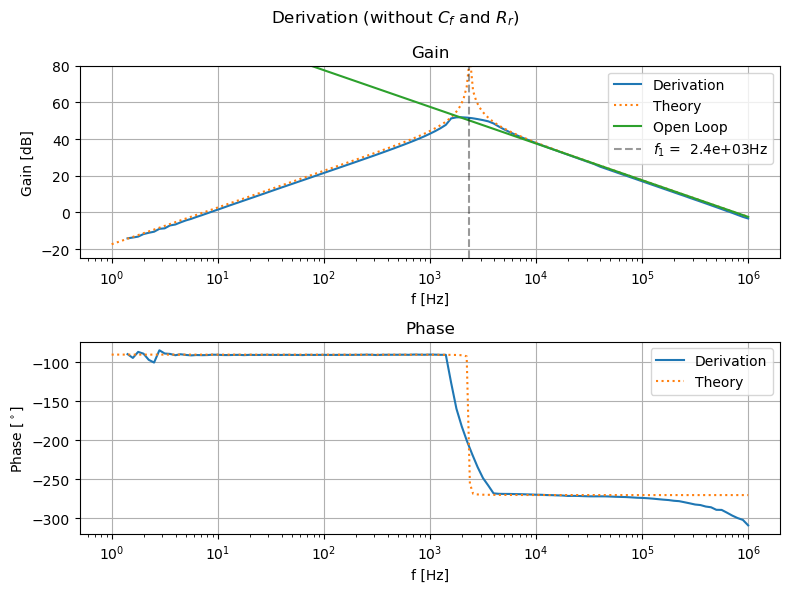
\includegraphics[width=0.8\columnwidth]{./images/dervamp2_bode.png}
    \caption{$R_r$と$C_f$を抜いた微分回路の周波数応答}
    \label{fig:dervamp2_bode}
\end{figure}
図\ref{fig:dervamp2_bode}は$R_r$と$C_f$を抜いた微分回路の周波数応答の実測値(実線)と理論値(破線)である。
振幅特性の$\SI{2.4}{kHz}$付近にピークが存在するが、理論値と実測値で大きく値がずれている。
これは、ブレッドボードまたはオシロスコープの特性上、$\SI{15}{V}$までの電圧しか観測できないことによると思われる。
また、このとき$\zeta=0.0024$と、小さな値を示した。
また、位相の変化は理論値より緩やかであったが、これは寄生抵抗による$\zeta$の増大によるものだと考えられる。
高周波領域で再び位相のずれが観測されたが、これはたびたび考察しているように寄生インダクタンスと考えられる。
高周波領域では開ループ特性と一致するが、これは節\ref{sec:invertamp_theory}で述べたように、$A(s)$が小さい領域での$\frac{v_o}{v_i}$のゲインは$A(s)$に張り付くためである。

\subsection{$C_f$を抜いた場合の応答の理論値}
次に、$C_f$を抜いた。このとき、
\begin{equation*}
    Z_1 = R_r+\frac{1}{sC_r},\quad Z_2 = R_f
\end{equation*}
となる。このとき、
\begin{align}
    \alpha &= \frac{Z_2}{Z_1} \nonumber \\
    &= \frac{sR_fC_r}{1+\frac{s}{\omega_1}}
\end{align}
であり、これは$C_f$を入れたときの$\alpha$の、分母の$1+\frac{s}{\omega_2}$を除いたものである。
すなわち、$\alpha$自体は$f_1$でカットオフするHigh Pass特性を示す。
また、高周波では$A(s)$が小さくなるので、$A(s)$を上限とするような特性を示すはずである。

\subsection{$C_f$を抜いた場合の応答の実測値}
\begin{figure}[htbp]
    \centering
    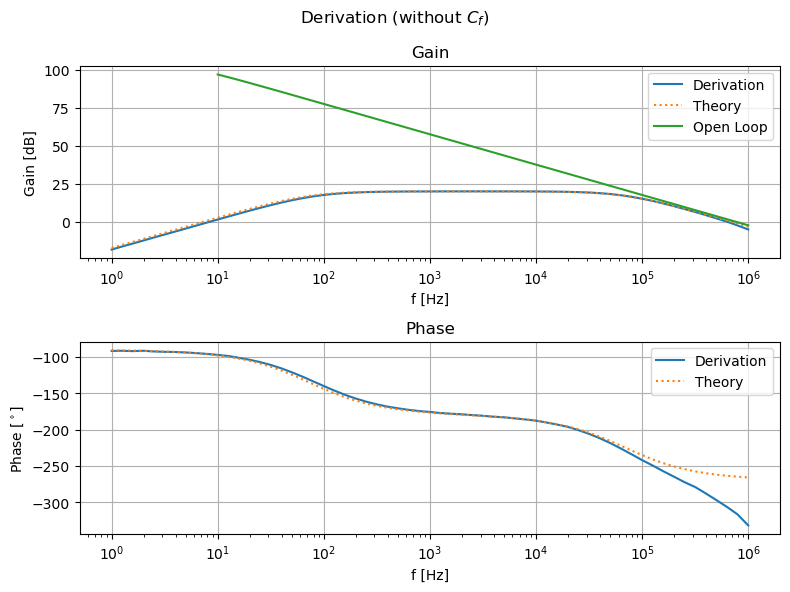
\includegraphics[width=0.8\columnwidth]{./images/dervamp3_bode.png}
    \caption{$C_f$を抜いた微分回路の周波数応答}
    \label{fig:dervamp3_bode}
\end{figure}
図\ref{fig:dervamp3_bode}は$C_f$を抜いた微分回路の周波数応答の実測値(実線)と理論値(破線)である。
位相特性が寄生インダクタンスの影響を受ける高周波領域で一致していない以外は理論値通りである。

\section{ウィーンブリッジ回路}
\subsection{理論値の計算}
\begin{figure}[htbp]
    \centering
    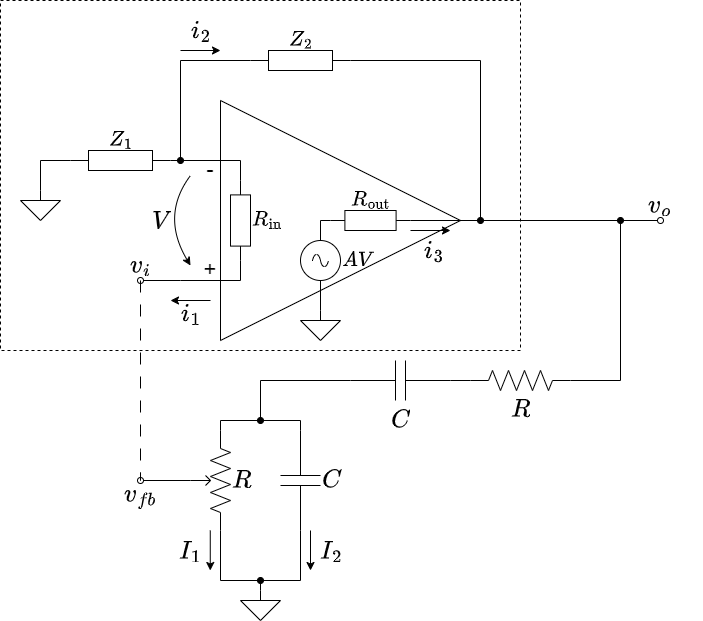
\includegraphics[width=0.8\columnwidth]{./images/wienbridge.png}
    \caption{ウィーンブリッジ回路の回路図}
    \label{fig:wienbridge_circuit}
\end{figure}
図\ref{fig:wienbridge_circuit}はウィーンブリッジ回路の回路図である。
図からわかるように、ウィーンブリッジ回路は非反転増幅回路の入力$v_i$に出力$v_o$をフィードバックする回路である。
このとき、フィードバック部分の伝達関数は以下のようにして求められる。
\begin{align}
    v_o &= \left( R+\frac{1}{sC}+\frac{R}{1+sRC} \right)(I_1+I_2) \\
    v_{fb} &= kRI_1 \\
    RI_1 &= \frac{1}{sC}I_2
\end{align}
このとき、
\begin{equation}
    \frac{v_{fb}}{v_o} = \frac{k(RCs)}{(RCs)^2+3(RCs)+1}
\end{equation}
となる。
また、フィードバックによる増幅率は、最初の信号を$\epsilon(s)$、オペアンプの伝達関数$\frac{v_o}{v_i}=A(s)$、フィードバックの伝達関数$\frac{v_{fb}}{v_o}=H(s)$とすると、
\begin{align}
    v_o &= \epsilon(s)A(s)\left( 1+A(s)H(s)+\left( A(s)H(s) \right)^2 + \dots \right) \nonumber \\
    \Leftrightarrow \frac{v_o}{\epsilon(s)} &= \frac{A(s)}{1-A(s)H(s)} \nonumber \\
    &= A\frac{(RCs)^2+3RCs+1}{(RCs)^2+(3-kA)RCs+1}
\end{align}
このとき、$3-kA<0\Leftrightarrow k>3/A$のとき、右半面に極が存在する、すなわち発散する。
今、$A=\frac{Z_1+Z_2}{Z_1}\approx10$であるから、$k\approx0.3$より大きい場合発散してしまう。
\begin{figure}[htbp]
    \centering
        \begin{minipage}{0.48\columnwidth}
            \centering
            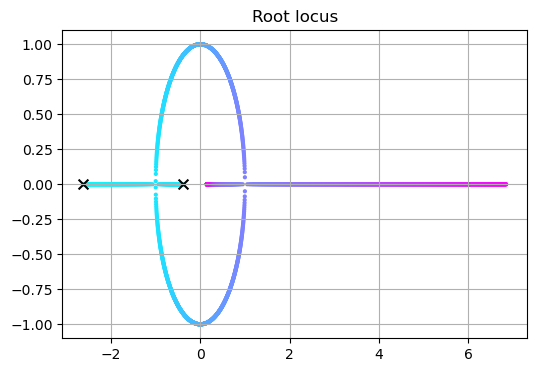
\includegraphics[width=0.95\columnwidth]{./images/wienbridge_rl.png}
            \caption{増幅率の根軌跡}
            \label{fig:wienbridge_rl}
        \end{minipage}
        \begin{minipage}{0.48\columnwidth}
            \centering
            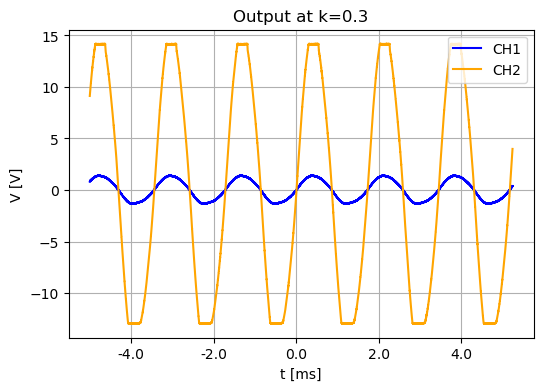
\includegraphics[width=0.95\columnwidth]{./images/wienbridge_response.png}
            \caption{ウィーンブリッジ回路の発散付近の応答}
            \label{fig:wienbridge_response}
        \end{minipage}
\end{figure}
図\ref{fig:wienbridge_rl}は、$RC=1$として$k$を変化させたときの増幅率の根軌跡である(水色がkが小さく、紫色が大きい)。
kが大きくなると分母の根(=極)は右に、すなわち発散が速くなっていくことがわかる。

\subsection{実測値}
\begin{figure}[htbp]
    \centering
    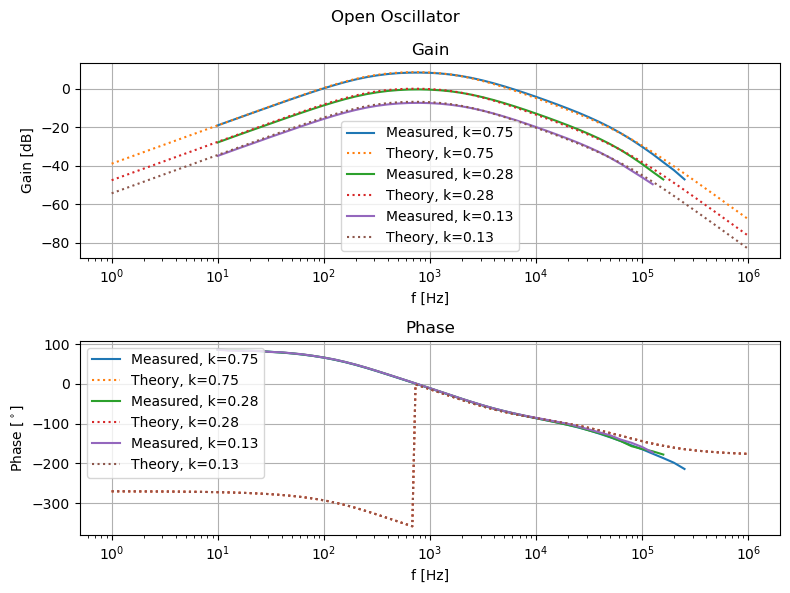
\includegraphics[width=0.8\columnwidth]{./images/wienbridge_bode.png}
    \caption{ウィーンブリッジ回路の開ループの周波数応答}
    \label{fig:wienbridge_bode}
\end{figure}
図\ref{fig:wienbridge_bode}はウィーンブリッジ回路の開ループの周波数応答の実測値(実線)と理論値(破線)である。
開ループ特性の理論値と実測値は、寄生インダクタンスの影響が大きい高周波以外では一致していた。

図\ref{fig:wienbridge_response}はウィーンブリッジ回路の発散付近での応答である。
実際、$R=\SI{2.97}{k\ohm}$、すなわち$k\approx0.3$で発散の開始が確認された。

\begin{figure}[htbp]
    \centering
        \begin{minipage}{0.48\columnwidth}
            \centering
            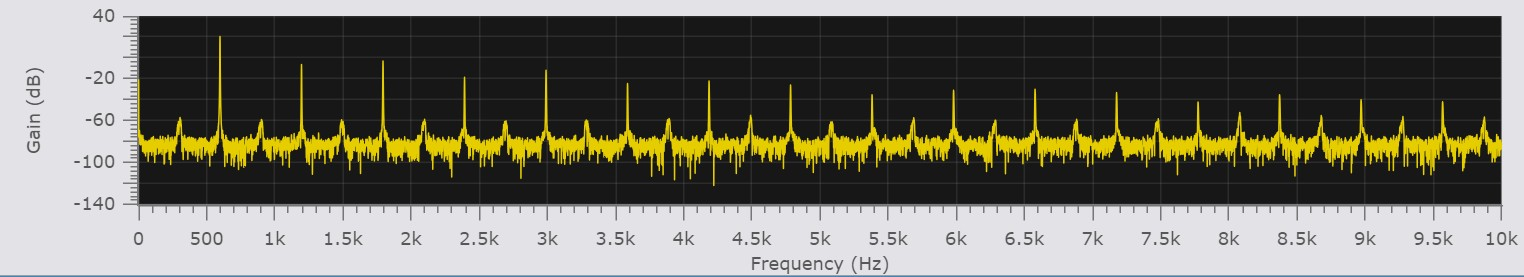
\includegraphics[width=0.95\columnwidth]{./images/wienbridge_spec_shallow.jpg}
            \subcaption{$\SI{2.9}{k\ohm}$($k=0.29$)でのスペクトル}
            \label{fig:wienbridge_spec_shallow}
        \end{minipage}
        \begin{minipage}{0.48\columnwidth}
            \centering
            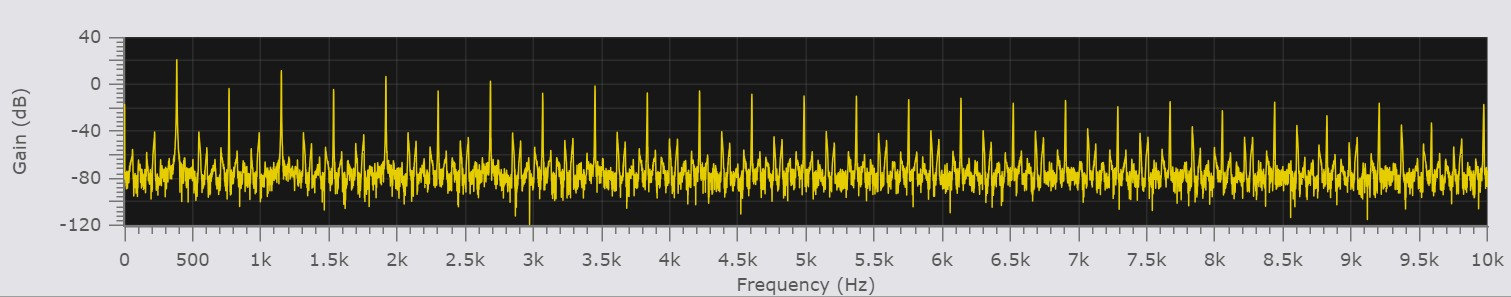
\includegraphics[width=0.95\columnwidth]{./images/wienbridge_spec_deep.jpg}
            \subcaption{$\SI{7.3}{k\ohm}$($k=0.73$)でのスペクトル}
            \label{fig:wienbridge_spec_deep}
        \end{minipage}
    \caption{異なる$k$でのスペクトルの違い}
    \label{fig:wienbridge_spec}
\end{figure}
図\ref{fig:wienbridge_spec}は、異なる$k$でのスペクトルの違いである。
図から見て分かるように、$k$が大きいほど周波数が小さくなっている。これは、根軌跡上を$k$が大きくなるにつれて縦に狭まっているからであると考えられる。


\begin{thebibliography}{99}
    \bibitem{Opamp offset} オペアンプ オフセットの調整方法. (n.d.). Marutsu. Retrieved July 13, 2024, from \url{https://www.marutsu.co.jp/contents/shop/marutsu/mame/104.html}
    \bibitem{uA741} µA741 General-Purpose Operational Amplifiers. (2018). [Dataset]. Texas Instruments. \url{https://www.ti.com/lit/ds/symlink/ua741.pdf}
\end{thebibliography}

\end{document}